\subsection{Expressivity of ANIMO models}\label{sec:animo-drosophila}
Results obtained with ANIMO are comparable to results with other modeling
approaches. To demonstrate this, Figure~\ref{subfig:drosophila-model}
represents an ANIMO model of the circadian clock in \emph{Drosophila Melanogaster}, based on the work
by~\cite{drosophila-ode-model}, where ordinary differential equations (ODEs) were used.
The cyclic behavior of the circadian clock is based on the alternating formation and destruction of the
CYC/CLK protein complex.
Concentration levels of this complex are in turn regulated by a series of proteins which are produced as
a consequence of CYC/CLK formation. The CWO protein
is central to the functioning of the network, as it degrades the mRNA for most of the involved proteins.
As such, CWO act as an inhibitor that counterbalances the effect of CYC/CLK.
The positive influence of the light-regulated cryptochrome CRY on the degradation of TIM is a consequence
of the passage between day and night, allowing
the circadian clock to synchronize to a time zone (see Suppl. Sect.~\ref{suppl:repressilator}).


\def\drosophilaGraphScale{0.069}%0.123}

\begin{figure}[!htpb]
\begin{center}
\subfloat[\label{subfig:drosophila-model}]{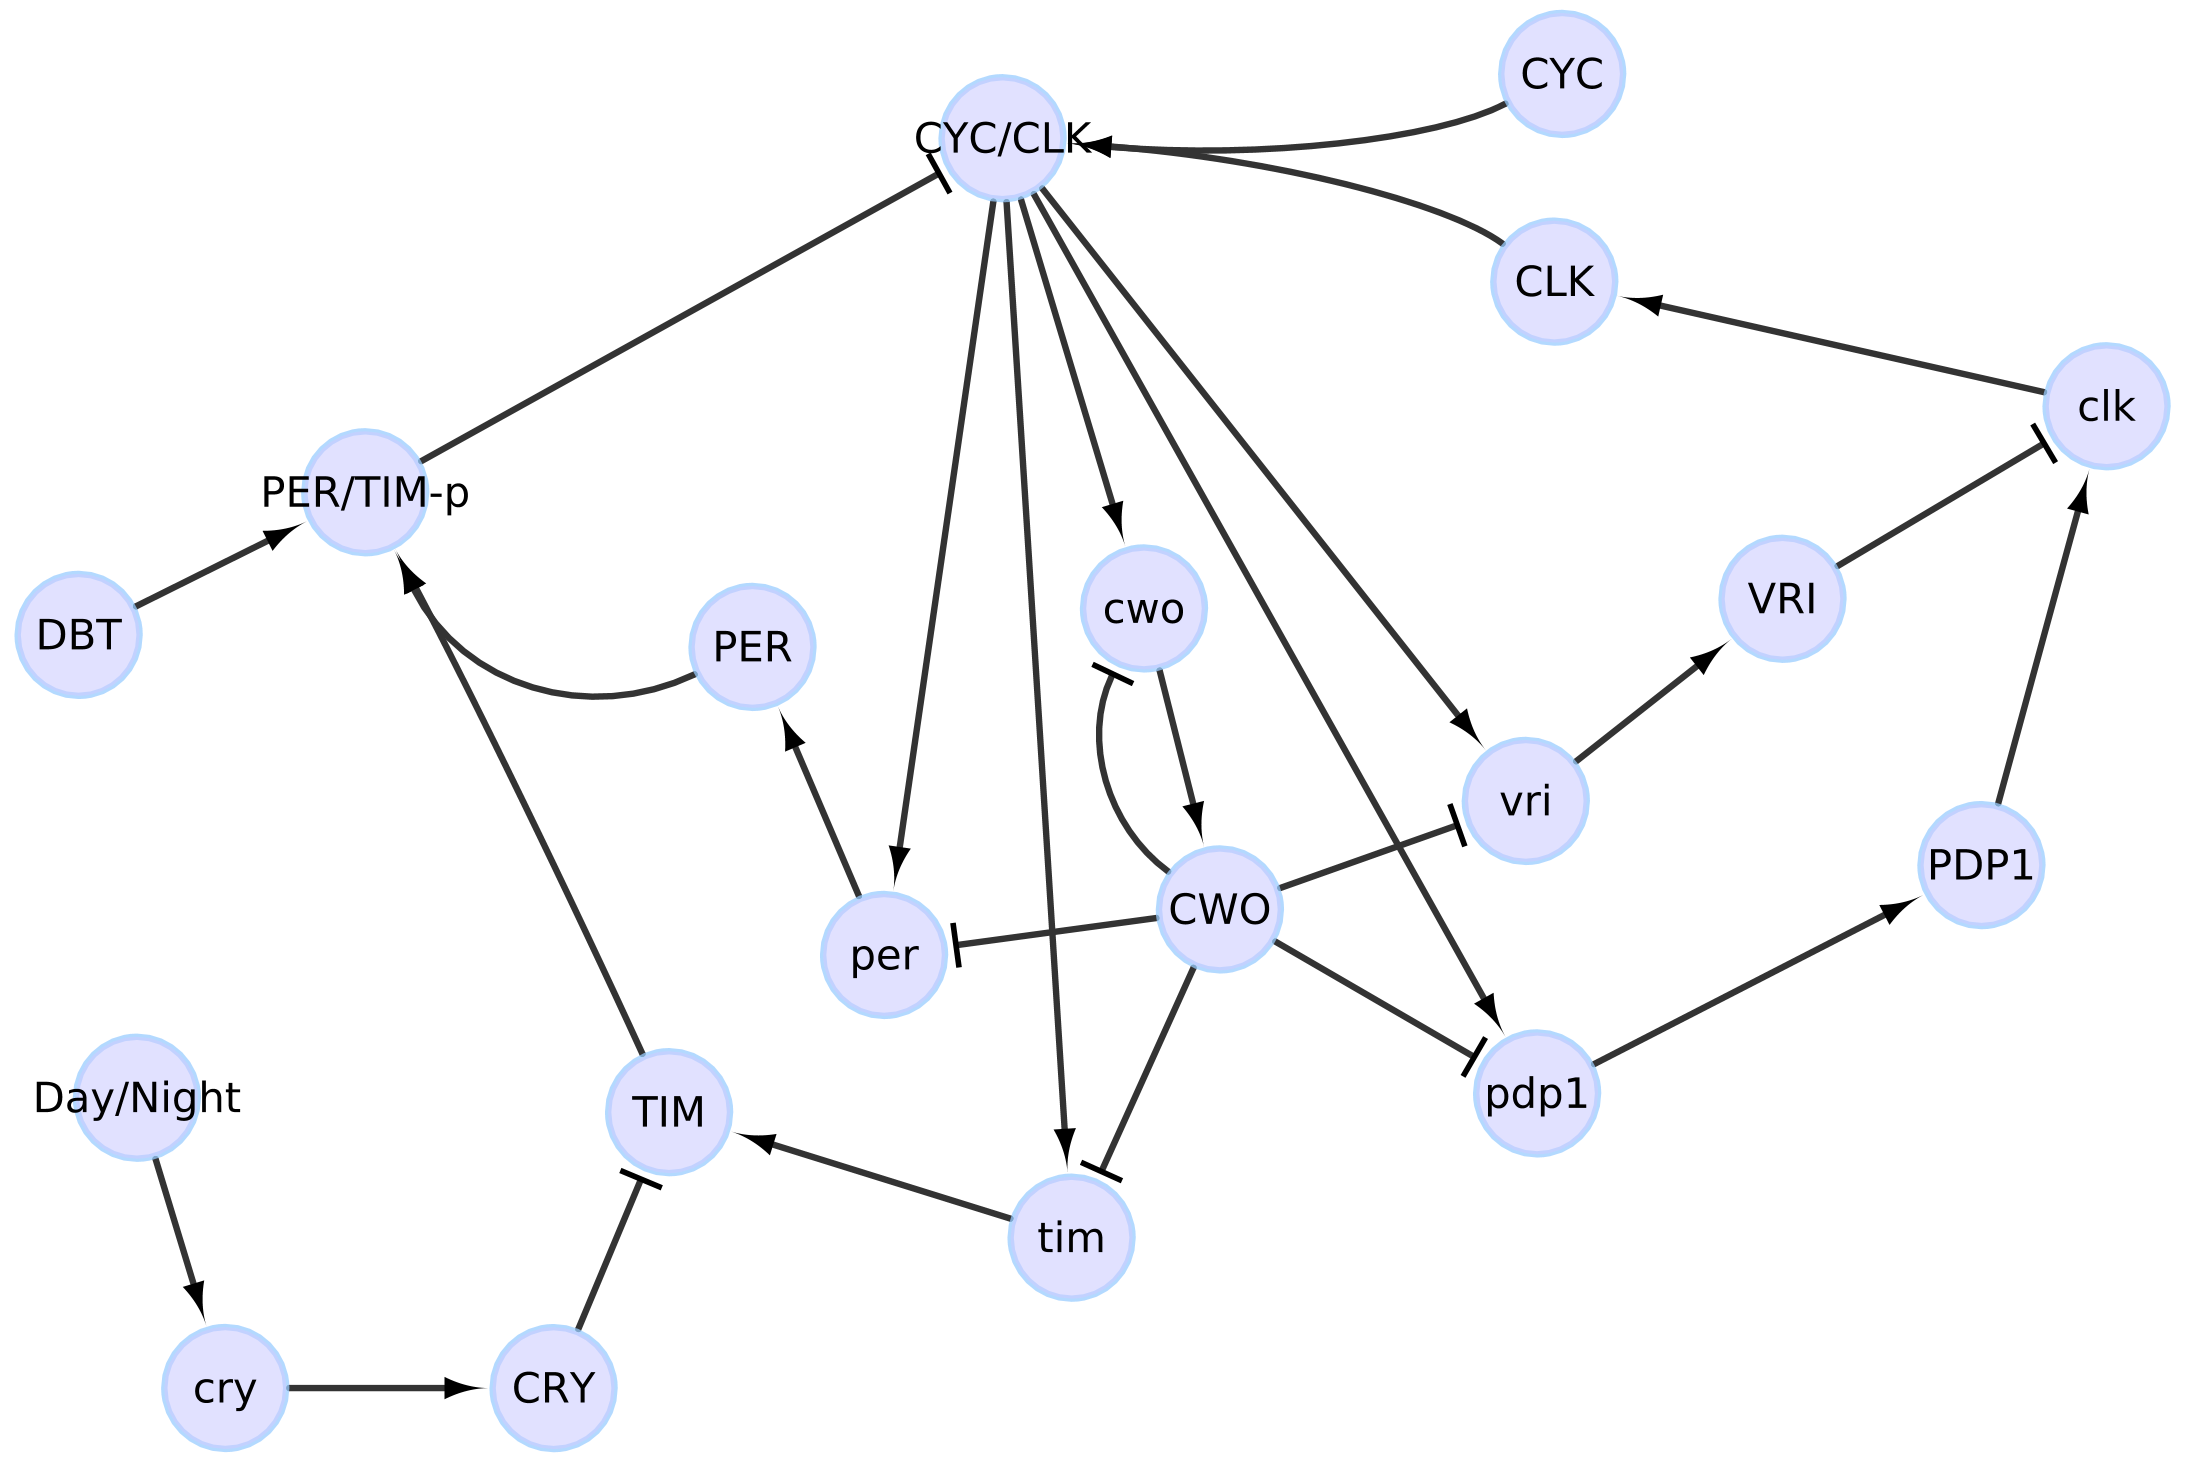
\includegraphics[width=0.49\textwidth]{images/drosophila_model5}}\ %0.85\textwidth
\subfloat[\label{subfig:drosophila-mrna}]{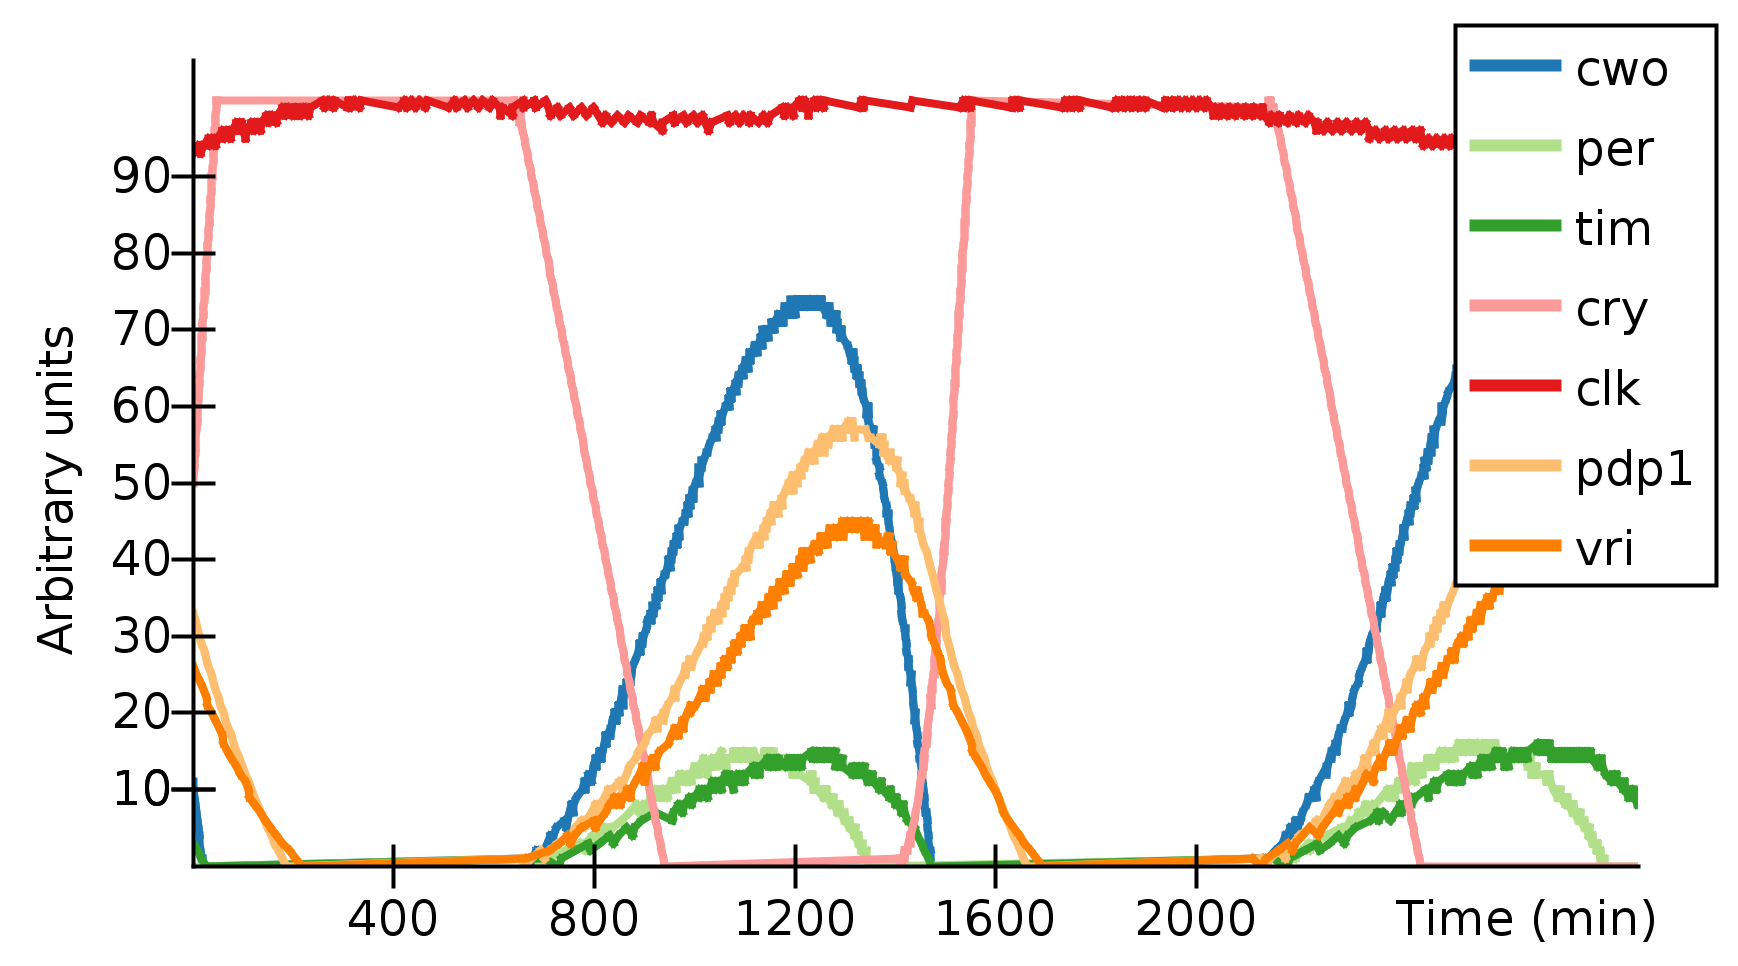
\includegraphics[scale=\drosophilaGraphScale]{images/drosophila_graph2}}\
\subfloat[\label{subfig:drosophila-proteins}]{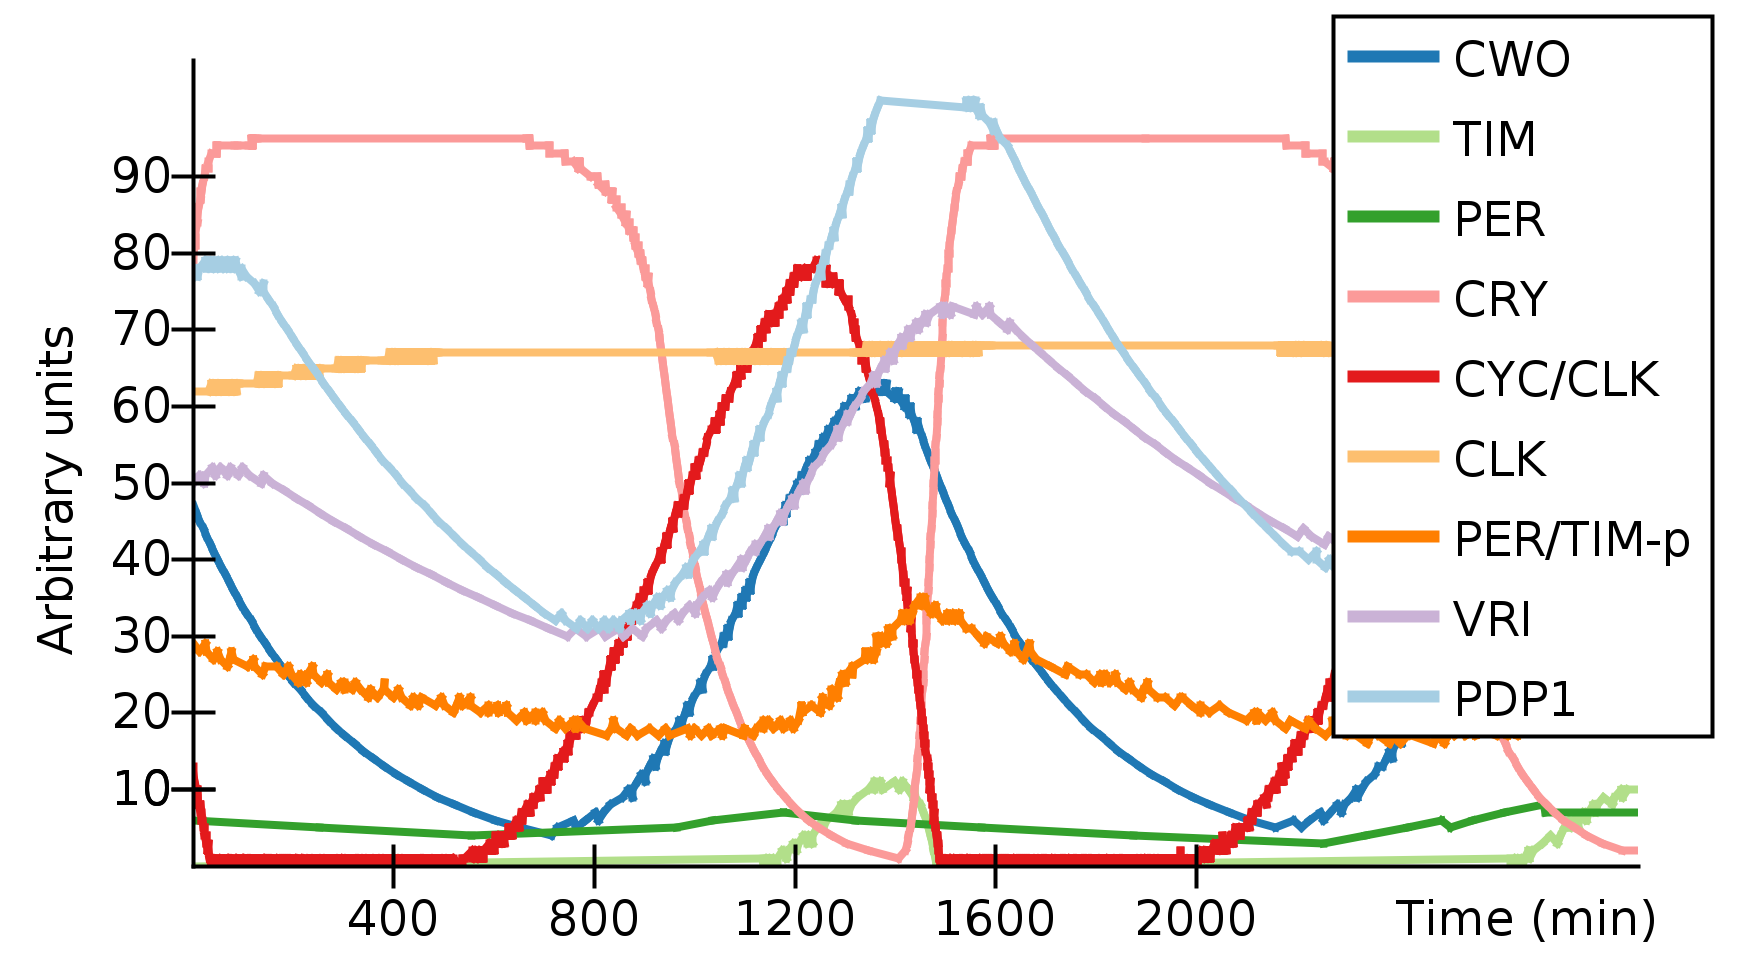
\includegraphics[scale=\drosophilaGraphScale]{images/drosophila_graph1}}
\end{center}
\caption{ANIMO model of the circadian clock in \emph{Drosophila Melanogaster} {\bfseries \protect\subref{subfig:drosophila-model}}.
Network topology of the ANIMO model. Autoregulatory negative feedback loops are present on each of the nodes of
the network, following the original model by~\cite{drosophila-ode-model}. These feedback loops ensure that
protein levels decrease over time, when activating inputs are absent. The feedback loops are not represented here
for cosmetic reasons and clarity.\\% Model parameters for nodes and interactions can be found in Supplementary Section~\ref{suppl-sec:animo-drosophila}.\\
ANIMO plots of the concentration of
mRNA~{\bfseries \protect\subref{subfig:drosophila-mrna}}
and proteins~{\bfseries \protect\subref{subfig:drosophila-proteins}} over a period of 48~hours.\\
Naming conventions follow the same rules
as in the original model, with lower-case names representing mRNA, and upper-case names indicating proteins.
}\label{fig:drosophila}
\end{figure}


The output of the ANIMO model in Figure~\ref{fig:drosophila} closely matches the original ODE model.
In particular, the oscillations in both models show the same periods and phases.
Due to the compositional nature of \tas\, ANIMO allows for intuitive \emph{in silico} knock-out experiments,
by right-clicking a node in the model and disabling it. Such experiments have been done
before~\citep{drosophila-ode-model} and give similar results in our model. Details of the comparison
between the ANIMO model and the original ODE model is given in Supplementary Section~\ref{suppl-sec:animo-drosophila}.



\subsection{Case study: using ANIMO to generate hypotheses}\label{subsec:case-study-larger}
In order to validate our modeling approach,
we constructed a larger model of the signaling network downstream of TNF$\alpha$ and EGF, formalizing
the crosstalk that takes place between the pathways at different levels of cellular regulation.
We first modeled the two pathways in isolation~(Figs.~\ref{fig:large-model-tnf}, \ref{fig:large-model-egf}),
using information on protein interactions from
the KEGG~\citep{kegg} and phosphosite~\citep{phosphosite} databases. These models were fitted to experimental data
from studies by~\citet{pathway-compendium} and~\citet{pathway-autocrine}.
We then merged the two pathways into a single model and added autocrine crosstalk between the pathways that has been
described by~\citet{pathway-autocrine}.
Briefly, stimulation with TNF$\alpha$ leads to a rapid release of TGF$\alpha$ ({\sf TGFa} in the model),
which activates the EGF receptor ({\sf EGFR}).
This activation causes secretion of IL-1$\alpha$ ({\sf IL-1a}) at later time points.
The effect of IL-1$\alpha$ is down-regulated by the secretion of IL-1 receptor antagonist ({\sf IL-1ra})
downstream of TNF$\alpha$.
The resulting model (Fig.~\ref{fig:large-model-no-hypotheses}) was compared to the experimental data
for treatments with 100 ng/ml TNF alone and 100 ng/ml EGF alone (data not shown)~\citep{pathway-compendium}.

At this point, the behavior of the model deviated from the data for some of the nodes.
This is an interesting situation, as it requires
modifications to the model, that can be interpreted as new hypotheses. Below, we give two examples and show how
adaptation of the model can be used to generate novel testable hypotheses.



\def\largeModelScale{0.18}%0.15}%0.155}%0.27}
\def\legendScalaColori{0.21}%0.18}%0.21}
\def\legendScalaForme{0.21}%0.18}%0.21}
\def\scalaGrafici{0.0709}%0.13}
\begin{figure}[!htpb]
\centering
 \subfloat[\label{fig:large-model-no-hypotheses}]{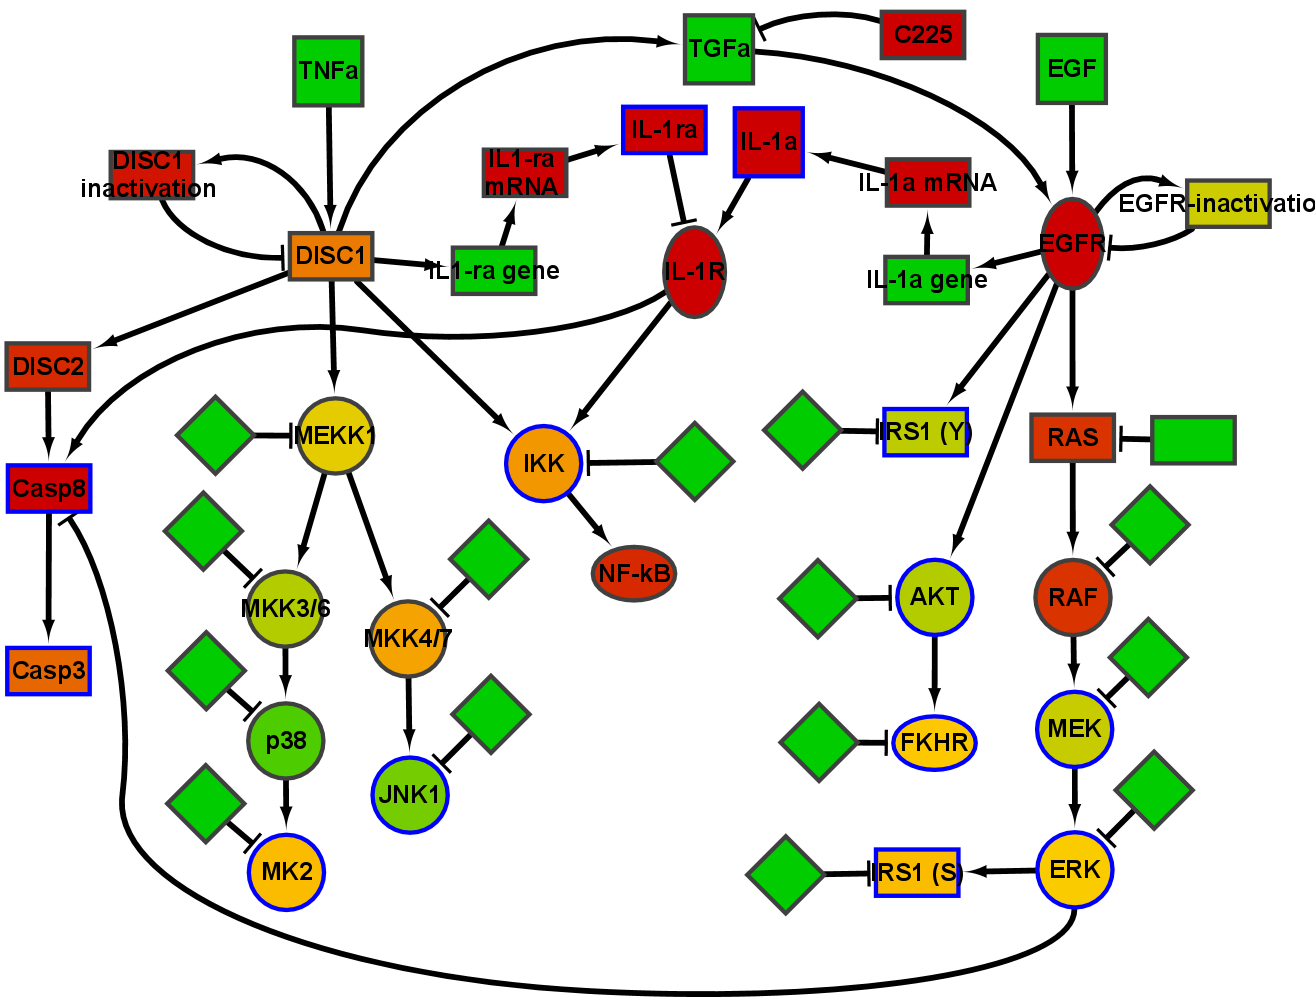
\includegraphics[scale=\largeModelScale]{images/large_network_merged_no_hypotheses}}\\
%\subfloat{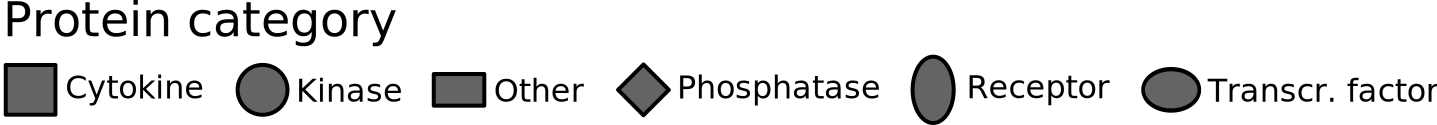
\includegraphics[scale=\legendScalaColori]{images/legenda_forme}}\\ \subfloat{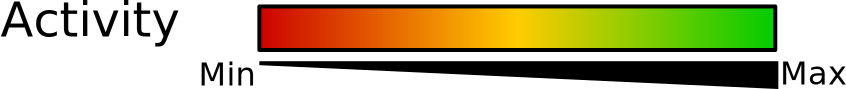
\includegraphics[scale=\legendScalaForme]{images/legenda_colori}}\\
\subfloat{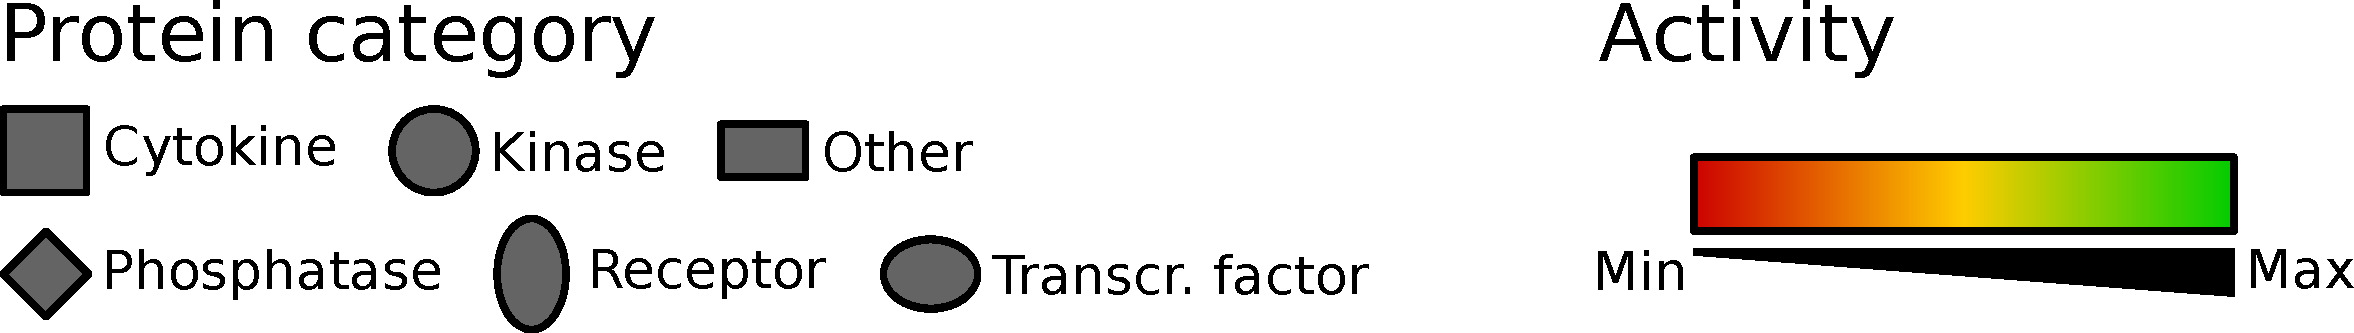
\includegraphics[scale=\legendScalaColori]{images/legenda_forme_e_colori}}\\
\addtocounter{subfigure}{-1}
\subfloat[\label{fig:large-model-graph1}]{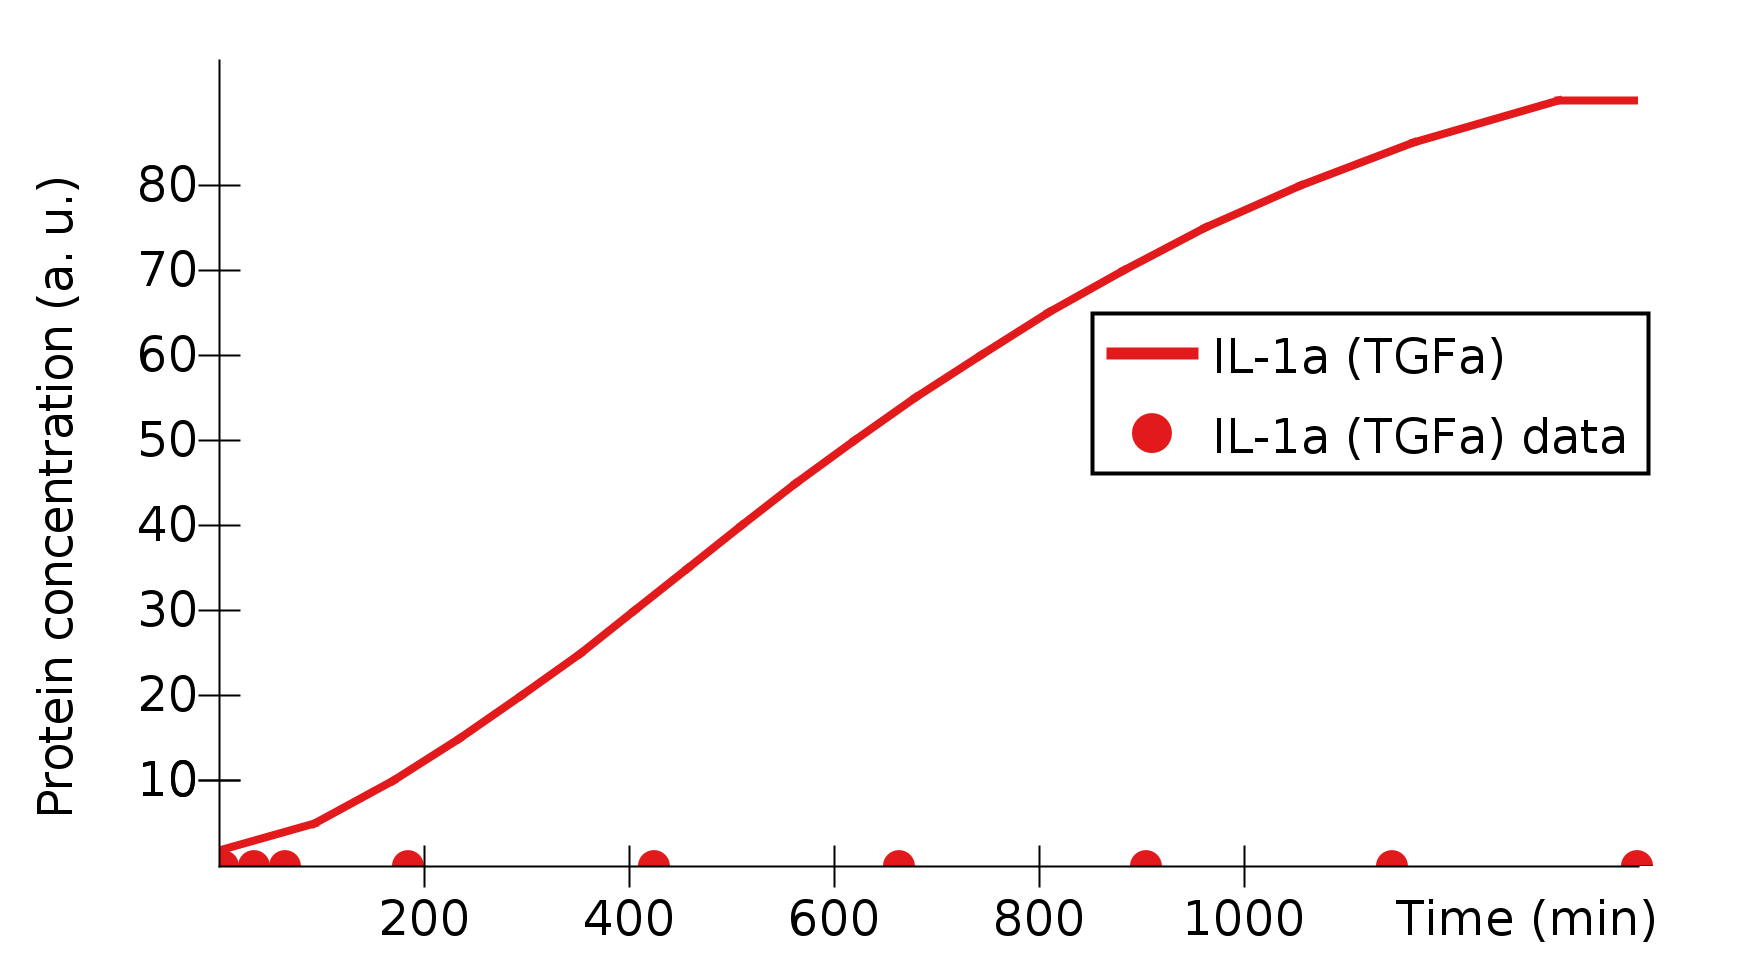
\includegraphics[scale=\scalaGrafici]{images/TGF100_TNF0_ho_hyp_IL-1a3}}
\subfloat[\label{fig:large-model-graph3}]{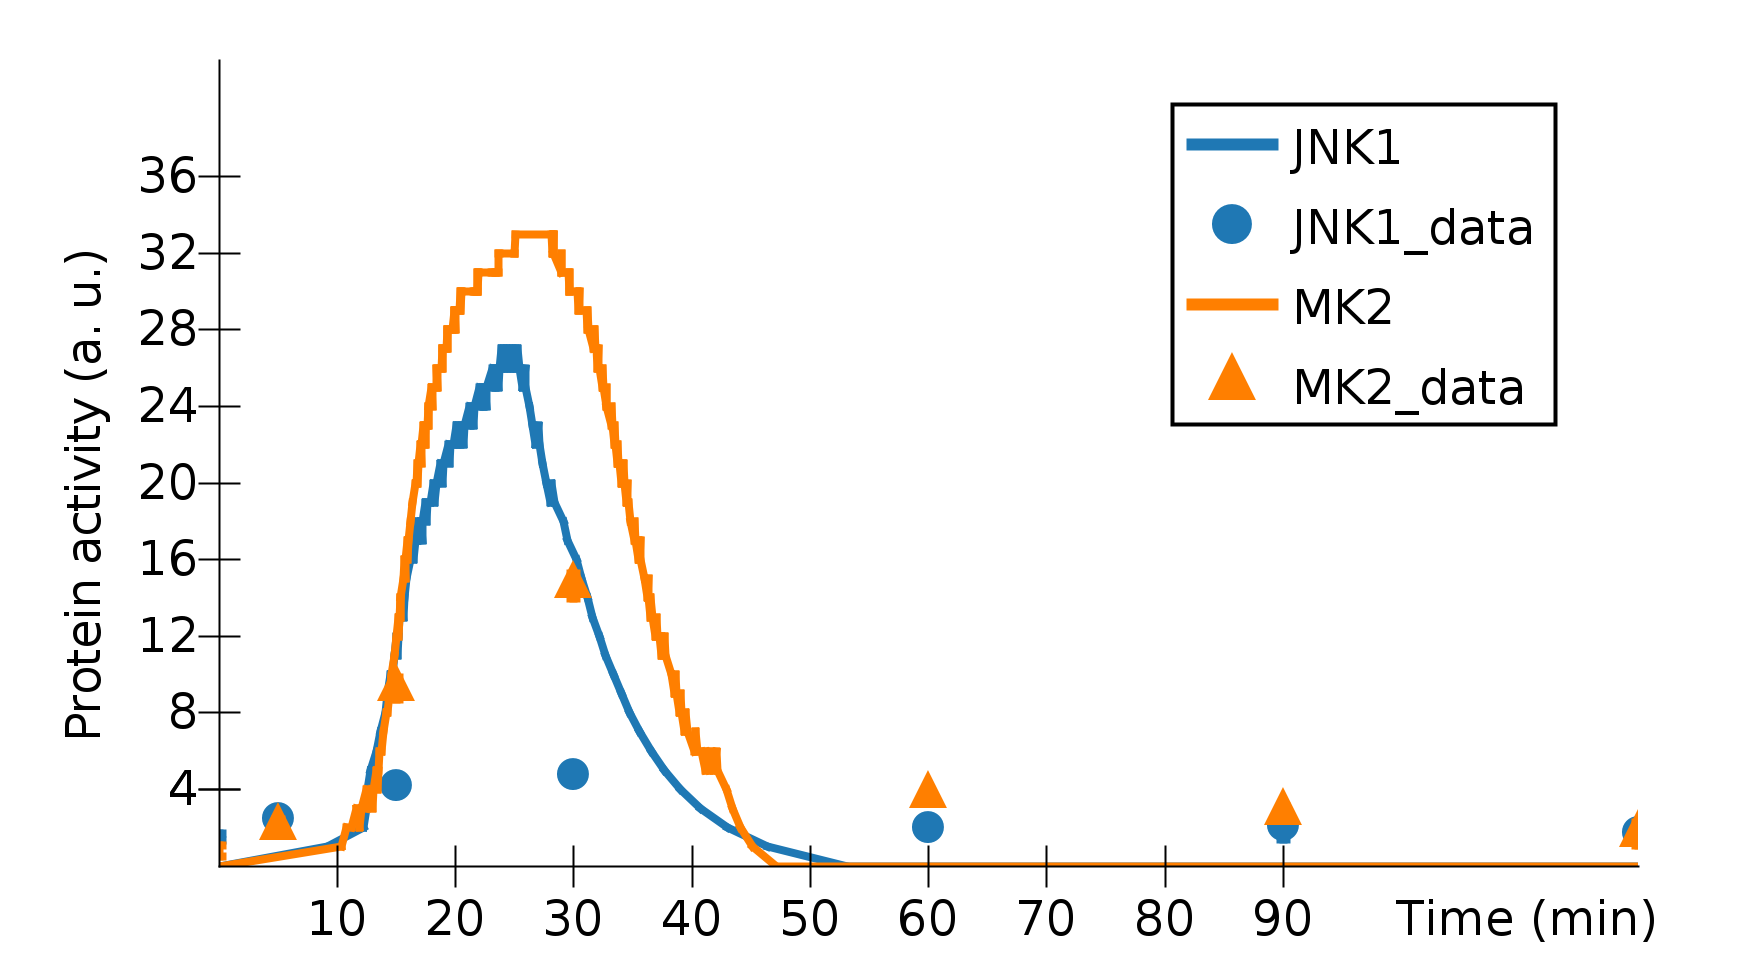
\includegraphics[scale=\scalaGrafici]{images/TNF5_C225_no_hyp_JNK1_MK2}}
\caption{Signalling network downstream of TNF$\alpha$ and EGF in human colon carcinoma cells.
{\bf \protect\subref{fig:large-model-no-hypotheses}}
The model for the merged TNF$\alpha$ and EGF pathways. Node colours represent the
activity level of the corresponding modelled reactants at time $t = 15$ minutes after
a stimulation of 100 ng/ml TNF$\alpha$ + 100 ng/ml EGF.
{\bf \protect\subref{fig:large-model-graph1}}~Modelled production of IL-1$\alpha$ after stimulation with 100 ng/ml TGF$\alpha$ (24 hours).
{\bf \protect\subref{fig:large-model-graph3}}~Modelled activation of JNK1 and MK2 after stimulation with 5 ng/ml TNF$\alpha$ + 10 $\mu$g/ml C225 (2 hours).
}\label{fig:large-model-all}
\end{figure}


Experimentally,
treatment with TGF$\alpha$ alone does not lead to secretion of IL-1$\alpha$. Instead, a co-stimulation with
TGF$\alpha$ and TNF$\alpha$ is required~\citep{pathway-autocrine}.
However, in the first version of the model, treatment with TGF$\alpha$ was sufficient for
IL-1$\alpha$ expression (Fig.~\ref{fig:large-model-graph1}). Given the time delay until secretion of IL-1$\alpha$, it can be
expected that \emph{de novo} synthesis of IL-1$\alpha$ is required and that both
TNF$\alpha$ and TGF$\alpha$ are needed to activate transcription of the IL-1$\alpha$ gene.
JNK1 and ERK signal downstream of TNF$\alpha$ and TGF$\alpha$, respectively, and are known
to affect the activity of multiple transcription factors. We altered the model to make
activation of IL-1$\alpha$ expression dependent on both JNK1 activity and ERK activity
(Suppl. Fig.~\ref{fig:large-model-hypotheses}, arrows linking {\sf JNK1} and {\sf ERK} to {\sf IL-1a gene}).
After this modification to the model, IL-1$\alpha$ was no longer secreted
upon stimulation with TGF$\alpha$ alone, which greatly improved the fit between the measured IL-1$\alpha$
levels and the model (Fig.~\ref{fig:large-model-graph2}). This hypothesis could now be used to
design a new experiment to validate IL-1$\alpha$ as a target of combined JNK1 activity and ERK activity in
HT-29 cells. For example, kinase inhibitors specific to JNK1 and ERK could be used to confirm that activity of
both kinases is required for expression and secretion of IL-1$\alpha$. Performing the experiment is beyond
the scope of this study, but this hypothesis finds support in literature.
Transcription factors c-Jun and c-Fos together
form a heterodimer known as AP-1 and are activated by JNK1 and ERK,
respectively~\citep{jnk-signaling,cfos-cjun}. AP-1 has been reported to bind to the
promoter of IL-1$\alpha$, providing evidence for a role in the regulation of IL-1$\alpha$
expression~\citep{ap1-il1a}. Based on these findings in literature we included c-Jun and
c-Fos in our model as transcriptional activators of IL-1$\alpha$ (Fig.\ref{fig:large-model-complete}).

\begin{figure}[!tpb]
\begin{center}
\subfloat[\label{fig:large-model-complete}]{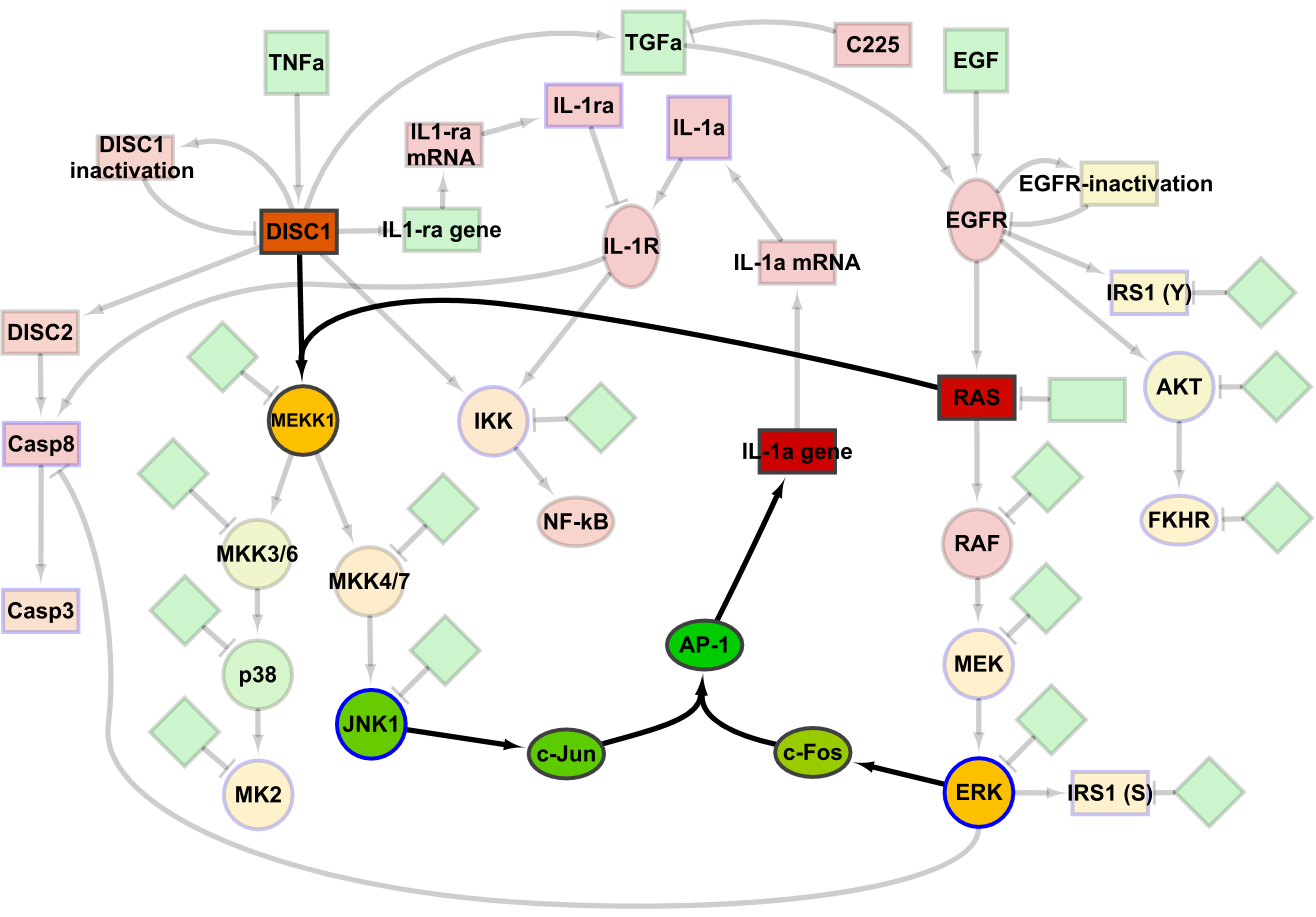
\includegraphics[scale=\largeModelScale]{images/large_network_legendg}}\\
 \subfloat[\label{fig:large-model-graph2}]{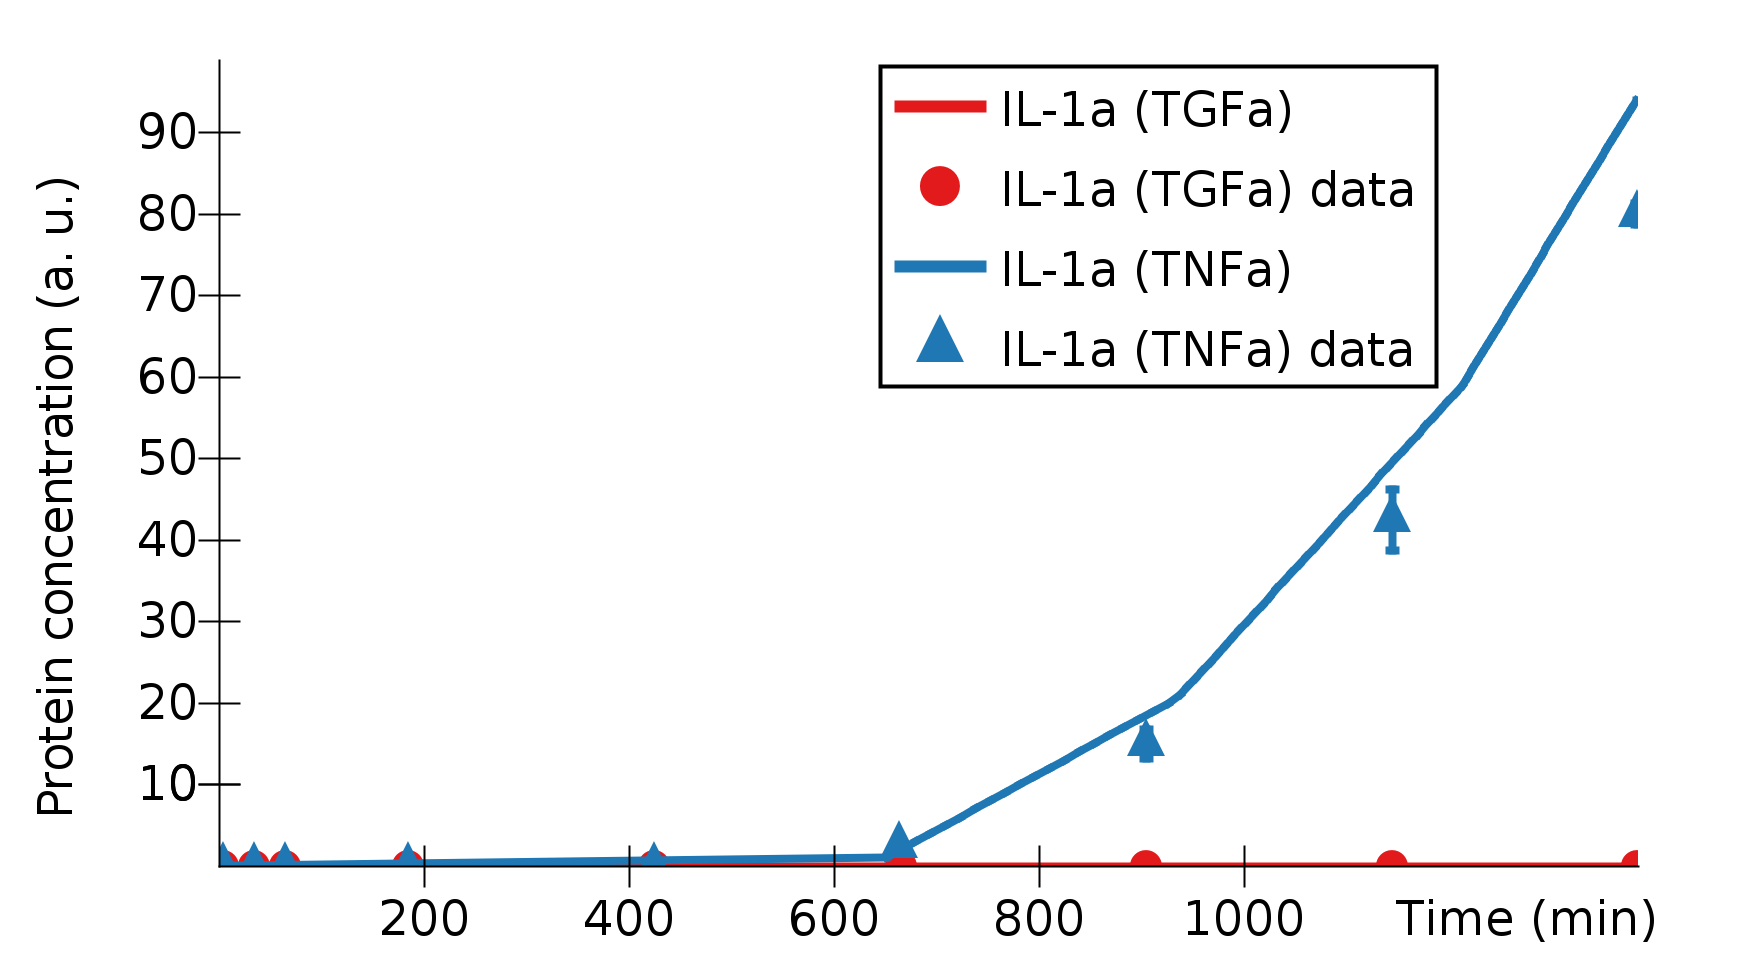
\includegraphics[scale=\scalaGrafici]{images/TGF100_vs_TNF100_hyp1_IL-1a4}}
 \subfloat[\label{fig:large-model-graph4}]{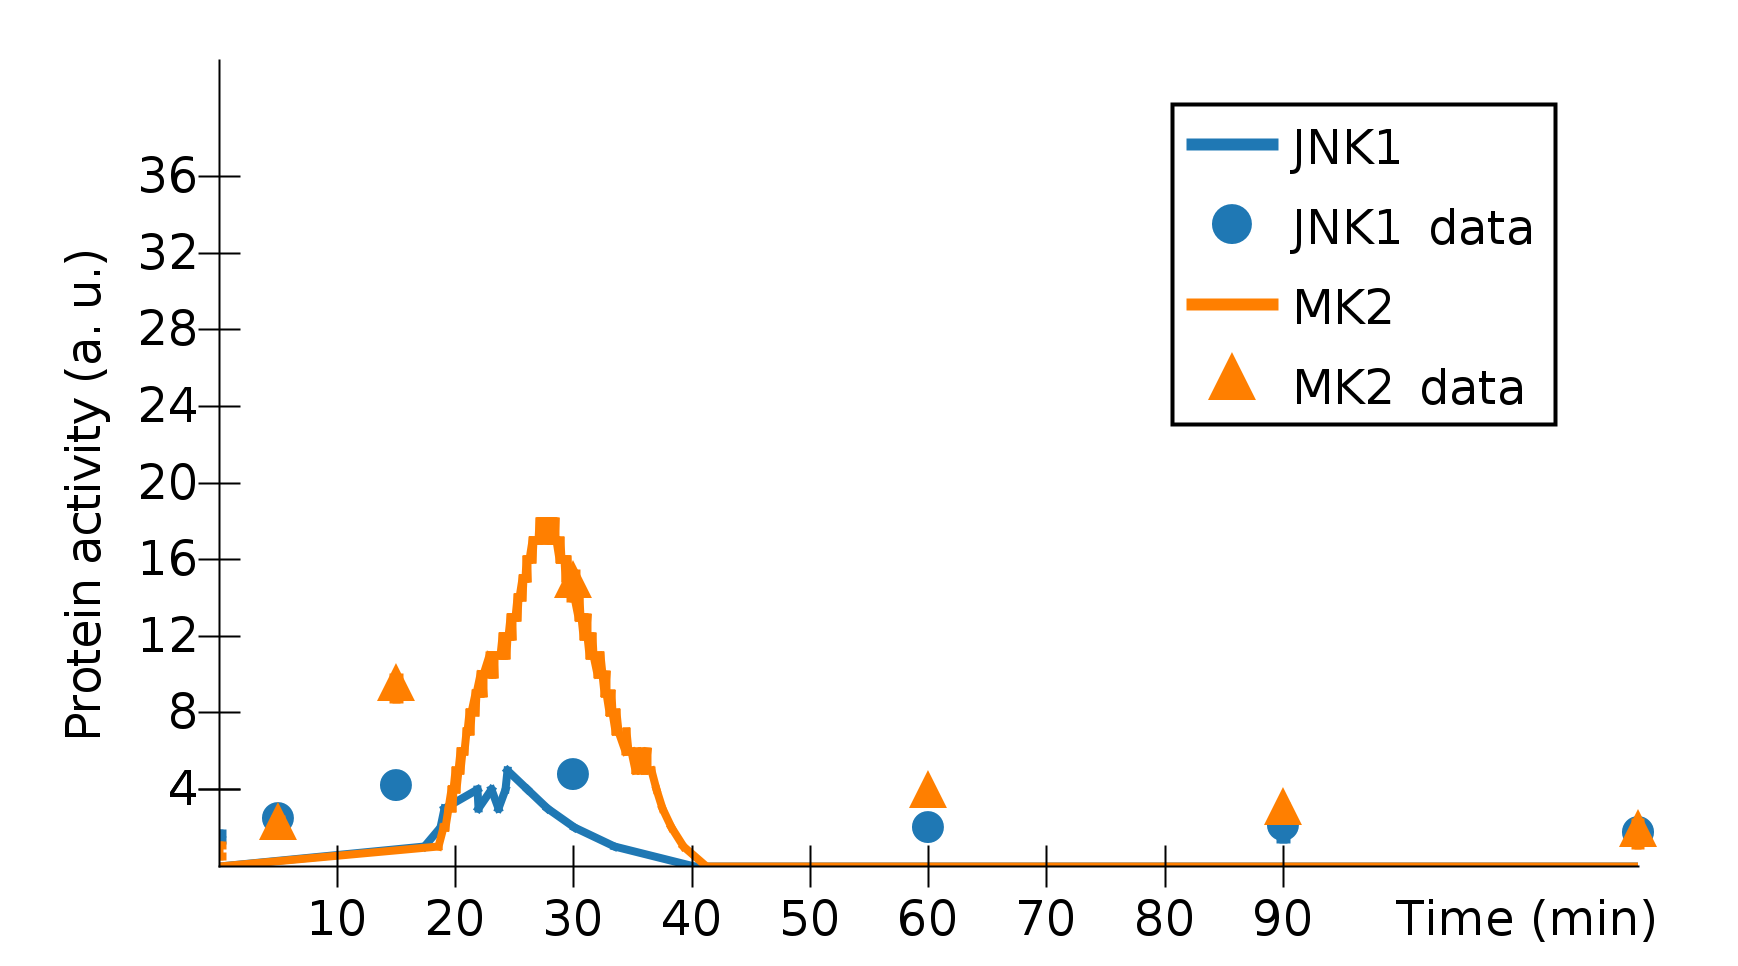
\includegraphics[scale=\scalaGrafici]{images/TNF5_C225_hyp2_JNK1_MK2}}
\end{center}
\caption{\scriptsize
{\bf \protect\subref{fig:large-model-complete}} The model for the merged TNF$\alpha$ and EGF pathways
after addition of the two hypotheses (highlighted).
Hypothesis 1 assumes IL-1$\alpha$ expression to depend on AP-1 activity, which in turn requires
both c-Jun en c-Fos to be activated by JNK1 and ERK, respectively. Hypothesis 2 assumes RAS as an activator
of MEKK1. Node colours represent the activity levels $15$ minutes
after stimulation of 100 ng/ml TNF$\alpha$ + 100 ng/ml EGF.
{\bf \protect\subref{fig:large-model-graph2}}~After the addition of the first hypothesis (activation of IL-1$\alpha$ production depending both
on JNK1 and ERK): production of IL-1$\alpha$ after stimulation with 100 ng/ml TNF$\alpha$ (series {\sf IL-1a~(TNFa)})
compared with stimulation with 100 ng/ml TGF$\alpha$ (series {\sf IL-1a~(TGFa)}) (24 hours).\\
{\bf \protect\subref{fig:large-model-graph4}}~After the addition of the second hypothesis (activation of MEKK1 downstream of EGFR):
stimulation with 5 ng/ml TNF$\alpha$ + 10 $\mu$g/ml C225 (2 hours).
Suppl. Sect.~\ref{suppl:parameters-tnf-egf} explains how the dosage of 5 ng/ml TNF$\alpha$ was represented in the model.}\label{fig:large-model-graph}
\end{figure}


As a second example, we considered the behaviour of JNK1 and MK2. In the model, both
proteins were located downstream of TNF$\alpha$ but not TGF$\alpha$ or EGF. Hence, the
model did not show an effect of C225, a pharmacological inhibitor of ligand-EGFR
binding, on activation of JNK1 or MK2 after stimulation with TNF$\alpha$. However, experimental
data show that C225 strongly reduces activation of JNK1 and MK2 upon stimulation with
TNF$\alpha$~\citep{pathway-autocrine}.
This fact is indicative of a role for EGFR in activation of JNK1 and MK2. Since both JNK1 and MK2
are located downstream of MEKK1, we hypothesized that activation
of MEKK1 is dependent on
both TNF$\alpha$-signalling and TGF$\alpha$-signalling. In the model we added a new
hypothetical node {\sf Hyp~2} (hypothesis~2) to link EGFR to MEKK1 (Suppl. Fig.~\ref{fig:large-model-hypotheses}).
This addition led to an improved fit of the model to the data upon treatment with TNF$\alpha$ + C225:
activation of both MK2 and JNK1 was strongly suppressed by C225 (Fig.~\ref{fig:large-model-graph4}).
Stimulation with EGF alone did not lead to activation of JNK1 and MK2.
These data support the validity of the modification to the model.
Further support for a link between EGFR and MEKK1 was found in literature. Specifically,
Ras has been reported as a direct activator of
MEKK1~\citep{ras-mekk1}. EGFR is a well-known and potent activator of Ras,
which is why it was already in our network~\citep{kegg}.
Other studies also report activation of JNK1 and phosphorylation of c-Jun downstream of Ras, which is consistent with
an interaction between Ras and MEKK1~\citep{cfos-cjun,ras-jnk1}.
Based on these findings, we adapted
our model by removing the {\sf Hyp~2} node and creating a direct interaction between Ras
and MEKK1 (Fig.~\ref{fig:large-model-complete}). Experimentally, the role of Ras could be confirmed by using a
pharmacological inhibitor of Ras activity, and measuring the effect of this inhibitor on the activation of JNK1 and MK2.
Together, our model suggests that EGFR activity is required
but not sufficient for activation of JNK1 and MK2 in HT-29 cells.


There are other nodes for which the experimental data deviates from the model in one or more of the experimental conditions.
A comparison between model and experimental data can be found in Figures~\ref{fig:differences1}, \ref{fig:differences2} and~\ref{fig:differences3}.
A complete deciphering of the signalling events
in this biological system is outside the scope of this paper. Instead, we illustrated how interactive modelling of the dynamic behaviour
of a signal transduction network can be used to extend previous pathway topologies and can lead to the generation of novel hypotheses.
